% 2007 春季上海 Q19 图2: 四块地砖绕中心旋转 90 度铺设, 四角灰三角, 中央深色四边形 EFGH
\usetikzlibrary{arrows.meta}
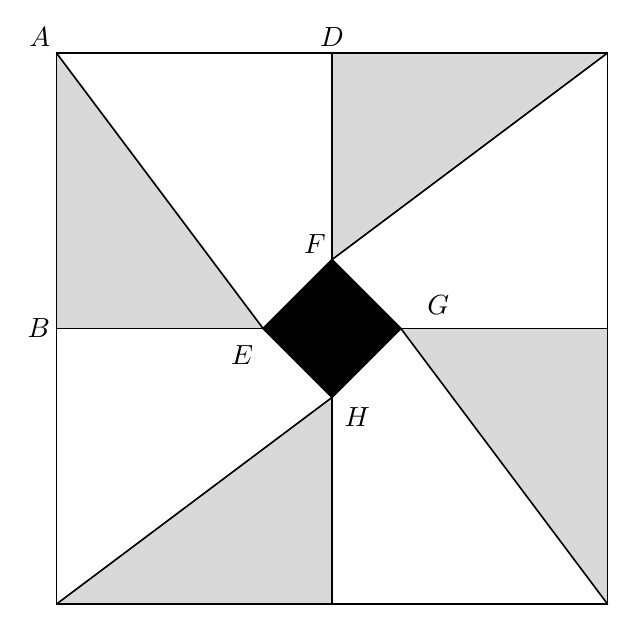
\begin{tikzpicture}[x=1cm,y=1cm,line width=.6pt,
  geometry edge/.style={line width=.6pt},
  geometry label/.style={inner sep=1pt}]
\coordinate (A) at (0,7);
\coordinate (TR) at (7,7);
\coordinate (BR) at (7,0);
\coordinate (BL) at (0,0);
\coordinate (Dtop) at (3.5,7);
\coordinate (Bmid) at (0,3.5);
\coordinate (Rmid) at (7,3.5);
\coordinate (Botmid) at (3.5,0);
\coordinate (E) at (2.625,3.5);
\coordinate (F) at (3.5,4.375);
\coordinate (G) at (4.375,3.5);
\coordinate (H) at (3.5,2.625);
% 四块地砖的灰色三角形 (ABE 型)
\fill[gray!30] (A)--(Bmid)--(E)--cycle;
\fill[gray!30] (TR)--(Dtop)--(F)--cycle;
\fill[gray!30] (BR)--(Rmid)--(G)--cycle;
\fill[gray!30] (BL)--(Botmid)--(H)--cycle;
% 中央深色四边形 EFGH
\filldraw[black] (E)--(F)--(G)--(H)--cycle;
% 外轮廓
\draw[geometry edge] (A)--(TR)--(BR)--(BL)--cycle;
% 中线
\draw[geometry edge] (Bmid)--(E);
\draw[geometry edge] (G)--(Rmid);
\draw[geometry edge] (Dtop)--(F);
\draw[geometry edge] (H)--(Botmid);
% 四条斜线 AE, TRF, BRG, BLH
\draw[geometry edge] (A)--(E);
\draw[geometry edge] (TR)--(F);
\draw[geometry edge] (BR)--(G);
\draw[geometry edge] (BL)--(H);
% 标签
\node[anchor=south east,inner sep=0pt,xshift=-2pt,yshift=2pt] at (A) {$A$};
\node[anchor=south,inner sep=0pt,yshift=2pt] at (Dtop) {$D$};
\node[anchor=east,inner sep=0pt,xshift=-2pt] at (Bmid) {$B$};
\node[anchor=south east,inner sep=0pt,xshift=-2pt,yshift=2pt] at (F) {$F$};
\node[geometry label,anchor=center] at (2.36,3.16) {$E$};
\node[geometry label,anchor=center] at (4.85,3.80) {$G$};
\node[geometry label,anchor=center] at (3.82,2.38) {$H$};
\end{tikzpicture}
